% default values
\def\ttau{1} % Zeitkonstante tau

% Plot Umgebung:
\def\samples{41}

\def\xomegaordermin{-2}
\def\xomegaordermax{+2}
\def\xomegamin{1e\xomegaordermin}
\def\xomegamax{1e\xomegaordermax}
\def\domain{\xomegamin:\xomegamax}

\def\yamptiefmin{0.8e-2}    % \ymin needed as macro to draw ycomb with node-text from x-axis to plot
\def\yamptiefmax{2}

\def\yamphochmin{0.8e-2}    % \ymin needed as macro to draw ycomb with node-text from x-axis to plot
\def\yamphochmax{2}

\def\yphitiefmax{+10}
\def\yphitiefmin{-100}      % \ymin needed as macro to draw ycomb with node-text from x-axis to plot % 1. Ordnung
\def\yphitiefg{-45}

\def\yphihochmin{-10}       % \ymin needed as macro to draw ycomb with node-text from x-axis to plot % 1. Ordnung % Alternative: [ycomb, update limits=false] small y value outer bounds but no dynamic node text
\def\yphihochmax{100}
\def\yphihochg{45}

%%%%%%%%%%%%%%%%%%%%%%%%%%%%%%%%%%%%%%%%%%%%%%%%%%%%%%%%%%%%%%%%%%%%%%%%%%%%

% RC-Tiefpass 1. Ord. Amplitudengang
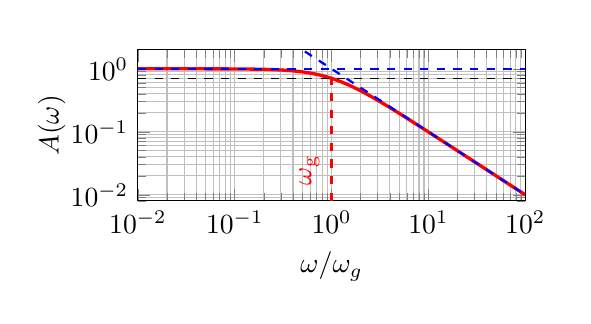
\begin{tikzpicture}[x=1mm,y=1mm] % gilt für tikz-coordinaten außerhalb der axis-environment
    \draw[draw=none] (-14,-12) rectangle (54,22); % Bildrahmen, Koordinatenbezug auf (0,0) des \begin{axis}...\end{axis} pgfplots, für
    \begin{axis}[
        %title={Amplitudengang RC-Tiefpass 1. Ordnung},
        xmode=log,ymode=log,
        xlabel={$\omega/\omega_g$},
        ylabel={$A(\omega)$},
        ylabel shift = -5 pt,
        xmin=\xomegamin, xmax=\xomegamax,
        ymin= 0.8 * 1/(1+(\xomegamax*\ttau)^2)^0.5, % 0.8*0.01 (manual cut off bottom)
        ymax=\yamptiefmax,   % \ymin needed as macro to draw ycomb with node-text from x-axis to plot intersection
        domain=\domain,
        samples=\samples,
        log origin=infty,%for ycomb
        width=6.5cm,
        height=3.5cm,
        grid=minor,
    ]     
    \addplot+[mark=none,very thick,red,]   {1/(1+(x)^2)^ 0.5}; % Plot

    \addplot+[ycomb,dashed,mark=none,thick,red,] coordinates { (1/(\ttau),\yamptiefmin) (1/(\ttau),1/2^0.5)} 
        node [pos=0.25,sloped,style={yshift=8pt}] {$\omega_{\mathrm{g}}$}; % Grenzfrequenz             
    \addplot+[dashed,mark=none,thick,blue] coordinates { (\xomegamin,1) (\xomegamax,1) }; % Asymptote
    \addplot+[dashed,mark=none,thick,blue]   { 1/(x*\ttau) }; % Asymptote
    \addplot+[dashed,mark=none,black,]  coordinates { (\xomegamin, 1/2^0.5) ( \xomegamax, 1/2^0.5) }; % 1/sqrt(2) Linie      

    \end{axis}
\end{tikzpicture}%